% !TEX program = xelatex
% =====================================================================
%  《新生实践课》课程实验报告
%  编译方式：XeLaTeX
% =====================================================================
\documentclass[12pt,a4paper,fontset=fandol]{ctexart}

% ---------------------------- 页面与字体 ----------------------------
\usepackage{geometry}
\geometry{a4paper,left=3.2cm,right=2.7cm,top=2.6cm,bottom=2.4cm,
          headheight=12pt,headsep=1.15cm,footskip=0.6cm}

\usepackage{graphicx}
\usepackage{url}
\def\UrlBreaks{\do\/}
\graphicspath{{images/}{shots/}{./}}
\usepackage{xcolor}
\usepackage{fancyhdr}
\usepackage{titlesec}
\usepackage{tocloft}
\usepackage{indentfirst}
\usepackage{enumitem}
\usepackage{caption}
\usepackage{booktabs}
\usepackage{array}
\usepackage{newunicodechar}
\usepackage{float}
\usepackage{tikz}
\counterwithin{figure}{section}
\counterwithin{table}{section}
\renewcommand{\thefigure}{\thesection-\arabic{figure}}
\renewcommand{\thetable}{\thesection-\arabic{table}}
\usetikzlibrary{arrows.meta,positioning}

% -------------------- 生僻字字体回退 --------------------
\makeatletter
\def\rarecjknone{NONE}
\let\rarecjkfile\rarecjknone
\IfFontExistsTF{bsmi00lp.ttf}{\def\rarecjkfile{bsmi00lp.ttf}}{%
  \IfFontExistsTF{bkai00mp.ttf}{\def\rarecjkfile{bkai00mp.ttf}}{%
    \IfFontExistsTF{rare-cjk.otf}{\def\rarecjkfile{rare-cjk.otf}}{}%
  }%
}
\ifx\rarecjkfile\rarecjknone\else
  \setCJKfamilyfont{rarecjk}{\rarecjkfile}[Scale=1.08]%
  \newunicodechar{屾}{{\CJKfamily{rarecjk}\char"5C7E}}%
\fi
\makeatother

\setmainfont{texgyretermes}[
  Extension      = .otf,
  UprightFont    = *-regular,
  BoldFont       = *-bold,
  ItalicFont     = *-italic,
  BoldItalicFont = *-bolditalic
]

% ---------------------------- 页眉页脚 ------------------------------
\pagestyle{fancy}
\fancyhf{}
\fancyhead[C]{\songti\fontsize{9}{11}\selectfont\color{black!55}%
  华\hspace{0.35em}中\hspace{0.35em}科\hspace{0.35em}技\hspace{0.35em}大\hspace{0.35em}学%
  \hspace{0.7em}课\hspace{0.35em}程\hspace{0.35em}实\hspace{0.35em}验\hspace{0.35em}报\hspace{0.35em}告}
\fancyfoot[C]{\songti\fontsize{10.5}{12}\selectfont\thepage}
\renewcommand{\headrulewidth}{0pt}
\renewcommand{\footrulewidth}{0pt}

\fancypagestyle{plain}{%
  \fancyhf{}%
  \fancyhead[C]{\songti\fontsize{9}{11}\selectfont\color{black!55}%
    华\hspace{0.35em}中\hspace{0.35em}科\hspace{0.35em}技\hspace{0.35em}大\hspace{0.35em}学%
    \hspace{0.7em}课\hspace{0.35em}程\hspace{0.35em}实\hspace{0.35em}验\hspace{0.35em}报\hspace{0.35em}告}%
  \renewcommand{\headrulewidth}{0pt}}
\fancypagestyle{tocpage}{%
  \fancyhf{}%
  \fancyhead[C]{\songti\fontsize{9}{11}\selectfont\color{black!55}%
    华\hspace{0.35em}中\hspace{0.35em}科\hspace{0.35em}技\hspace{0.35em}大\hspace{0.35em}学%
    \hspace{0.7em}课\hspace{0.35em}程\hspace{0.35em}实\hspace{0.35em}验\hspace{0.35em}报\hspace{0.35em}告}%
  \renewcommand{\headrulewidth}{0pt}}

% ---------------------------- 正文行距 ------------------------------
\linespread{1.31}
\setlength{\parskip}{0pt}

% 浮动体宽松度
\renewcommand{\topfraction}{0.95}
\renewcommand{\bottomfraction}{0.70}
\renewcommand{\textfraction}{0.05}
\renewcommand{\floatpagefraction}{0.96}
\setcounter{topnumber}{3}
\setcounter{bottomnumber}{2}
\setcounter{totalnumber}{4}

% ---------------------------- 章节标题 ------------------------------
\titleformat{\section}[hang]{\heiti\zihao{3}}{\thesection}{0.55em}{}
\titlespacing*{\section}{0pt}{4pt}{13pt}
\titleformat{\subsection}[hang]{\heiti\zihao{4}}{\thesubsection}{0.55em}{}
\titlespacing*{\subsection}{0pt}{13pt}{5pt}

% ---------------------------- 目录样式 ------------------------------
\renewcommand{\cfttoctitlefont}{\hfill\heiti\zihao{2}}
\renewcommand{\cftaftertoctitle}{\hfill}
\renewcommand{\cftsecfont}{\songti\zihao{-4}}
\renewcommand{\cftsecpagefont}{\songti\zihao{-4}}
\renewcommand{\cftsubsecfont}{\songti\zihao{5}}
\renewcommand{\cftsubsecpagefont}{\songti\zihao{5}}
\setlength{\cftbeforetoctitleskip}{6pt}
\setlength{\cftaftertoctitleskip}{18pt}
\setlength{\cftbeforesecskip}{9pt}
\setlength{\cftbeforesubsecskip}{5pt}
\setlength{\cftsecindent}{0pt}
\setlength{\cftsecnumwidth}{1.1em}
\renewcommand{\cftsecaftersnum}{\hspace{0.3em}}
\renewcommand{\cftsecleader}{\cftdotfill{\cftdotsep}}
\setlength{\cftsubsecindent}{1.7em}
\setlength{\cftsubsecnumwidth}{2.1em}
\renewcommand{\cftsubsecaftersnum}{\hspace{0.15em}}
\renewcommand{\cftsubsecleader}{\cftdotfill{\cftdotsep}}
\renewcommand{\cftdotsep}{1.4}

% ---------------------------- 图题与表题 ----------------------------
\DeclareCaptionFont{capfont}{\songti\fontsize{10.5}{14}\selectfont}
\captionsetup{font=capfont,labelfont=capfont,textfont=capfont,
  labelsep=space,skip=6pt}
\captionsetup[table]{position=bottom,skip=5pt}

% ---------------------------- 自定义命令 ----------------------------
\newlist{lablist}{enumerate}{1}
\setlist[lablist]{label=\arabic*),leftmargin=1.6em,labelsep=0.45em,
  topsep=0.3\baselineskip,itemsep=0.35\baselineskip,parsep=0pt}

\newcommand{\coverfield}[2]{%
  \makebox[2.65cm][r]{\songti\fontsize{15}{18}\selectfont #1}%
  \hspace{0.35em}%
  \underline{\makebox[7.2cm][c]{\heiti\fontsize{15}{18}\selectfont #2}}\par}

\begin{document}

% =====================================================================
%                              封  面
% =====================================================================
\thispagestyle{empty}

\vspace*{2.6cm}
{\centering
  {\heiti\fontsize{30}{36}\selectfont
   课\hspace{0.9em}程\hspace{0.9em}实\hspace{0.9em}验\hspace{0.9em}报\hspace{0.9em}告}\par}

\vspace{3.1cm}
{\centering
  \coverfield{课程名称：}{新生实践课}
  \vspace{0.78cm}
  \coverfield{专业班级：}{计算机2601班}
  \vspace{0.78cm}
  \coverfield{学\hspace{1em}号：}{U202614897}
  \vspace{0.78cm}
  \coverfield{姓\hspace{1em}名：}{陈镝屾}
  \vspace{0.78cm}
  \coverfield{指导教师：}{范晔斌}
  \vspace{0.78cm}
  \coverfield{报告日期：}{2026 年 11 月 19 日}\par}

\vspace{4.6cm}
{\centering
  {\heiti\fontsize{16}{19}\selectfont 计算机科学与技术学院}\par}

\newpage

% =====================================================================
%                              目  录
% =====================================================================
\thispagestyle{tocpage}
\tableofcontents
\newpage

% =====================================================================
%                              正  文
% =====================================================================
\setcounter{page}{1}

\section{网页整体框架}

本次课程实践的网站名为「个人网页」，是一个以自我介绍、课堂作业与日常记录为主线的静态站点，前后一共五个页面：首页、个人简介、动画作品、我的相册、学习心得，另加一张自定义的 404 页。站点已经发布在 GitHub Pages 上：主页 \url{https://facedes189.github.io/homework/}，仓库 \url{https://github.com/facedes189/homework}。

五个页面不是各写各的，我把它们当成同一副骨架换内容。从上往下依次是页头（站名、回到主页、日夜切换）、一段窄横幅（云、山丘、小屋和三只气球）、导航条（六个入口加一个点赞按钮）、正文的左右两栏（左栏放头像卡、页内目录和「今日一句」，右栏是真正的内容）、页脚（日期、三条快捷链接、一行探索成就）。骨架先定下来，之后改一处导航，五页一起变，不用逐页翻。网站整体框架如图 1-1 所示。

\begin{figure}[htbp]
  \centering
  \begin{tikzpicture}[
    font=\footnotesize,
    page/.style={draw=blue!55,fill=blue!5,rounded corners=3pt,
      minimum width=2.45cm,minimum height=1.0cm,align=center,inner sep=2pt},
    home/.style={page,fill=red!7,draw=red!55},
    ar/.style={-{Stealth[length=1.8mm]},draw=black!55}
  ]
    \node[draw=black!25,fill=black!3,rounded corners=3pt,
          minimum width=13.4cm,minimum height=0.8cm,align=center] (share) at (0,3.05)
      {共用样式 \texttt{css/style.css}　·　共用脚本 \texttt{js/main.js}　·　统一配色变量};

    \node[home] (home) at (0,1.5) {首页 \texttt{index.html}};
    \draw[ar] (share.south) -- (home.north);

    \node[page] (about)    at (-4.6,-0.6) {个人简介};
    \node[page] (works)    at (-1.55,-0.6) {动画作品};
    \node[page] (gallery)  at (1.55,-0.6)  {我的相册};
    \node[page] (thoughts) at (4.6,-0.6)   {学习心得};

    \draw[draw=black!45] (0,1.0) -- (0,0.45);
    \draw[draw=black!45] (-4.6,0.45) -- (4.6,0.45);
    \draw[ar] (-4.6,0.45) -- (-4.6,-0.05);
    \draw[ar] (-1.55,0.45) -- (-1.55,-0.05);
    \draw[ar] (1.55,0.45) -- (1.55,-0.05);
    \draw[ar] (4.6,0.45) -- (4.6,-0.05);

    \node[page,dashed,draw=black!35,fill=white,minimum width=1.5cm] (e404) at (6.95,1.5) {404};
  \end{tikzpicture}
  \caption{「个人网页」网站整体框架（虚线框为自定义 404 页，任何不存在的路径都会落到这里）}
\end{figure}

\begin{sloppypar}
结构上最花心思的是「共用」。样式集中在 \texttt{css/style.css}，脚本集中在 \texttt{js/main.js}，页面里只留结构。配色也只认几个变量：蓝 \#0b5fa5、红 \#e1553c、米白 \#fbf7f0，正文颜色另有三层灰。夜间模式没有另写一套样式，只是把变量换掉，所以后来每加一个板块，不必再改两遍。这件事我绕了一圈才明白：第一版是复制了一份 \texttt{style-night.css}，改到第三个页面就维护不动了，两边开始对不上。网站的文件组织如表 1-1 所示。
\end{sloppypar}

\begin{table}[htbp]
  \centering
  {\songti\fontsize{10.5}{15}\selectfont
  \begin{tabular}{@{}p{4.1cm}p{10.4cm}@{}}
    \toprule
    \heiti 文件 / 目录 & \heiti 说明 \\
    \midrule
    \texttt{index.html}     & 首页：问候语、本站一览、照片墙与四个入口 \\
    \texttt{about.html}     & 分页面 1「个人简介」：概况、联系方式、教育时间线、写信表单 \\
    \texttt{works.html}     & 分页面 2「动画作品」：四段纯 CSS 动画与参数滑块 \\
    \texttt{gallery.html}   & 分页面 3「我的相册」：六张手机照片的瀑布流与查看器 \\
    \texttt{thoughts.html}  & 分页面 4「学习心得」：三篇短文、页内目录与阅读进度 \\
    \texttt{404.html}       & 自定义 404：按层级反推站点根目录，保证深层地址样式不丢 \\
    \texttt{css/style.css}  & 全站样式：配色变量、日夜两套主题、栅格与动画 \\
    \texttt{js/main.js}     & 全站脚本：导航高亮、计数、查看器、便签、点赞 \\
    \texttt{images/}        & 自备素材：六张照片与站内插画 \\
    \bottomrule
  \end{tabular}}
  \vspace{-4pt}
  \caption{网站文件组织}
\end{table}

技术上一律用原生 HTML5、CSS3 和 JavaScript，没有引入任何框架、CDN 或第三方字体，因此断网也能完整打开。样式里用得最多的是 Grid 与 Flex：照片墙是三列不等高的网格，正文是左窄右宽的弹性两栏，窄屏时用两条媒体查询把它们叠成一栏。脚本做的是几件小事：按小时给页面打时间标记、进入视口时把数字从 0 数上去、相册的键盘翻页与焦点回位、便签的拖拽与本地存储。所有引用都是相对路径，整个文件夹原样拷到别的目录、或者直接双击 \texttt{index.html}，链接和图片都照常显示。

\section{主页设计}

首屏第一行不是标题，是一句问候，跟着电脑时间变：清晨「天刚亮，先喝口热水」，上午「脑子最清楚的时候」，午后、傍晚、深夜各有一句，过了十二点就催人睡觉。做法是脚本按小时给 \texttt{<html>} 打一个标记，CSS 决定显示哪一行，所以刷新时不会先闪一下再变。主页首屏如图 2-1 所示。

\begin{figure}[H]
  \centering
  
\includegraphics[width=12.8cm]{index.jpg}
  \caption{主页首屏（问候语随访问时间变化，右上角为日夜切换）}
\end{figure}

往下是「有朋自远方来，不亦乐乎」，右侧用几层很淡的同心圆压了个底纹。再往下「本站一览」四个数字——5 个页面、4 段动画、6 张照片、3 篇心得，进入视口时从 0 数上去。这一块第一版是写死的，摆在页面上像一块说明牌；改成计数以后，才有一点「这里是活的」的感觉。六张照片横排一行，点任意一张进相册；最下面四个纯文字链接，把四个分页面再引一遍。

整页只有蓝红两色点在米白上，留白多，晚上看不刺眼。我把配色收得很紧，是为了让照片成为页面上最花的东西；如果背景也用大面积渐变，六张手机照片压在上面就糊成一片了。导航条固定在顶部，滚动时始终可见，当前页的标签底下有一条短横线，靠脚本比对文件名加类名，不用每页手写。

\section{分页面设计}

四个分页面共用同一套页头、横幅和页脚，只在正文区做区分；导航条上的当前位置高亮、左栏的页内目录都由脚本按页面内容自动生成。下面按页面分别说明。

\subsection{个人简介}

\begin{figure}[H]
  \centering
  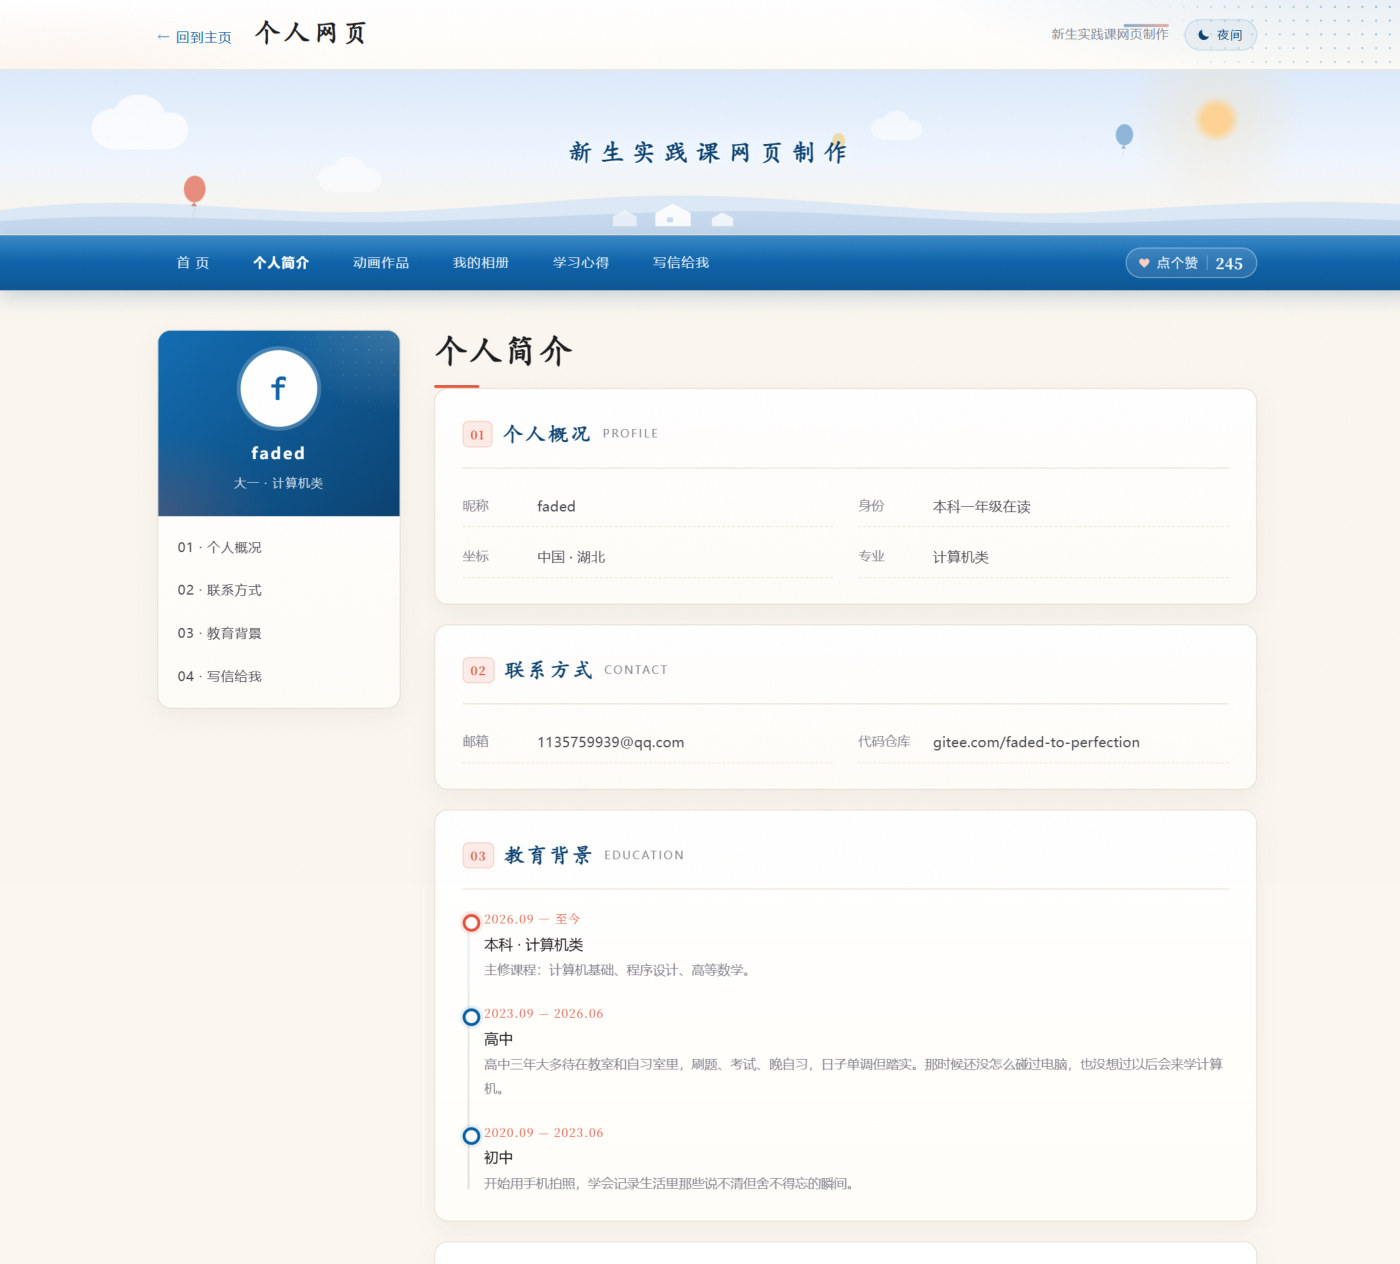
\includegraphics[width=12.8cm]{about.jpg}
  \caption{个人简介页（左侧锚点目录，右侧四块内容与便签墙）}
\end{figure}

四块内容：01 个人概况（昵称、身份、坐标、专业）、02 联系方式、03 教育背景（时间线，从初中写到现在）、04 写信给我；左上角一排锚点目录，点一下跳一段，滚动时当前项会自动加深。

「写信给我」原来是个 mailto 链接，点了会弹邮件客户端，很打断人。后来改成表单，提交后在本机生成一张手写体便签贴到下面的墙上，按住还能拖着换位置，位置存进浏览器本地存储，下次打开还在。便签不出本机，真想寄出去再点「用邮件寄一份」。页面如图 3-1 所示。

\subsection{动画作品}

\begin{figure}[H]
  \centering
  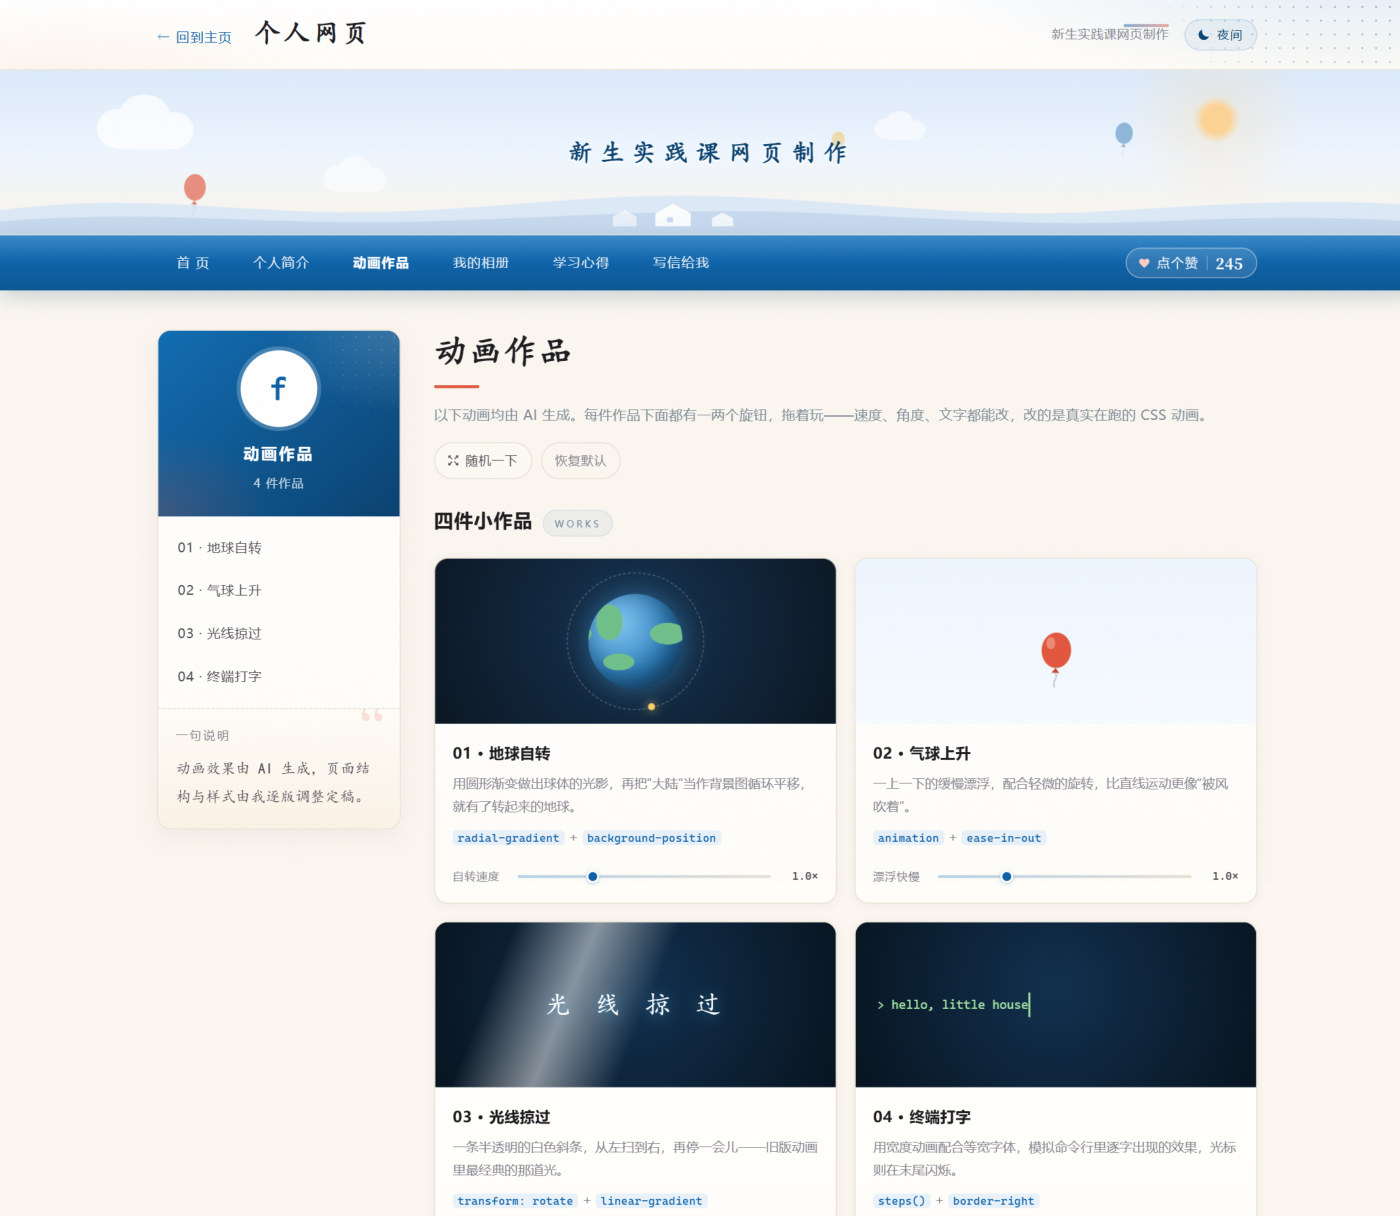
\includegraphics[width=12.8cm]{works.jpg}
  \caption{动画作品页（每段动画下方是调参滑块，拖动即时生效）}
\end{figure}

四段纯 CSS，没有一张动图、没有视频：地球自转用径向渐变做球面光影，再把「大陆」当背景图循环平移；气球上升是 ease-in-out 的上下浮动，带一点旋转，比直线运动更像被风吹着；光线掠过是一条半透明斜带从左扫到右，停一会儿再来；终端打字靠 \texttt{steps()} 逐字出现，光标用右边框闪烁。

每段下面有一两个滑块，拖的是 CSS 变量：转速、倾角、打字内容，改完立刻生效，能当场证明这些不是录屏。四段动画的初版是我让 AI 写的，然后一段段读懂、改参数改出来的；页面顶上那句「动画由 AI 生成，结构与样式由我逐版调整定稿」就写在明处，我觉得比藏着好。页面如图 3-2 所示。

\subsection{我的相册}

\begin{figure}[H]
  \centering
  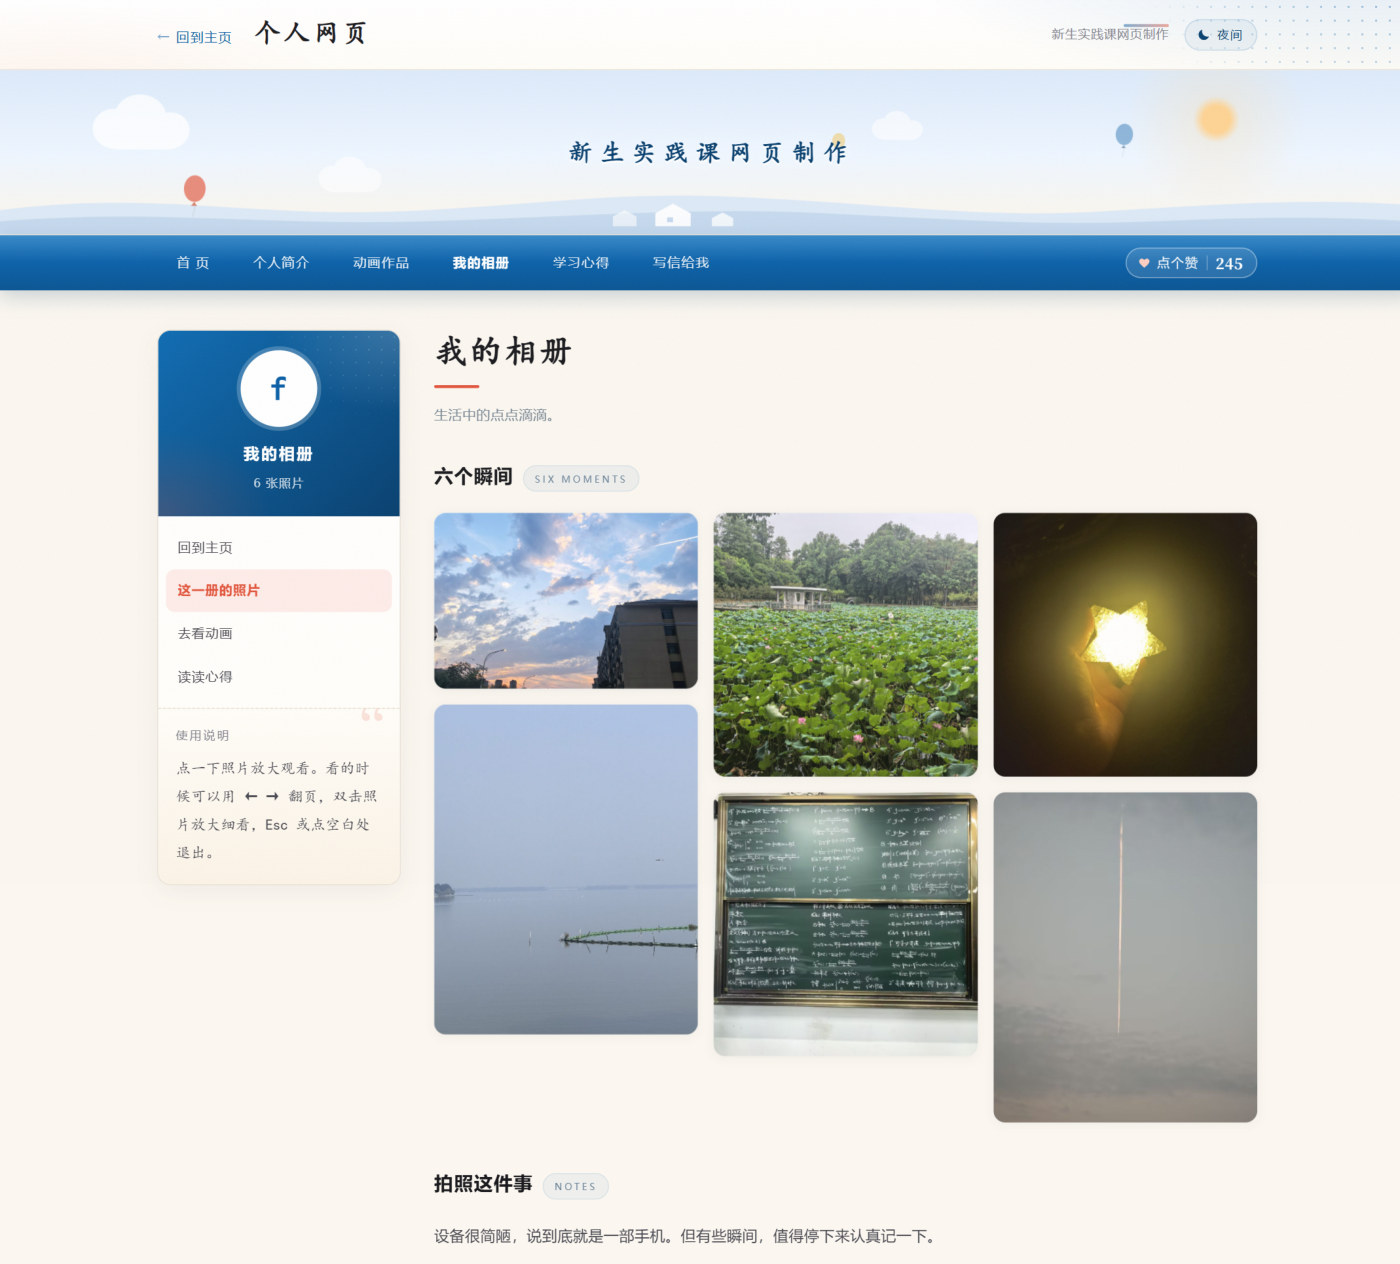
\includegraphics[width=12.8cm]{gallery.jpg}
  \caption{我的相册页（三列瀑布流，点开进入查看器）}
\end{figure}

六张都是手机拍的：傍晚的云、雾里的湖、荷叶池塘、写满公式的黑板、手里那颗发光的星、云层里划过的一道亮光。用 CSS 多列排成瀑布流，三列高度错开，进入视口时从「略大、略灰」落定，三列各差 0.08 秒，看着像依次显影。

点开是查看器：左右键翻页、底部缩略图直达、双击在 2.2 倍之间切换、Esc 或点空白关闭。关掉以后焦点会回到刚才那张照片——这一条是后来补的，用键盘翻到一半关掉，焦点跑回页首，很别扭。图片全部延迟加载，首屏只先取前两张，往下滚再取其余的。页面如图 3-3 所示。

\subsection{学习心得}

\begin{figure}[H]
  \centering
  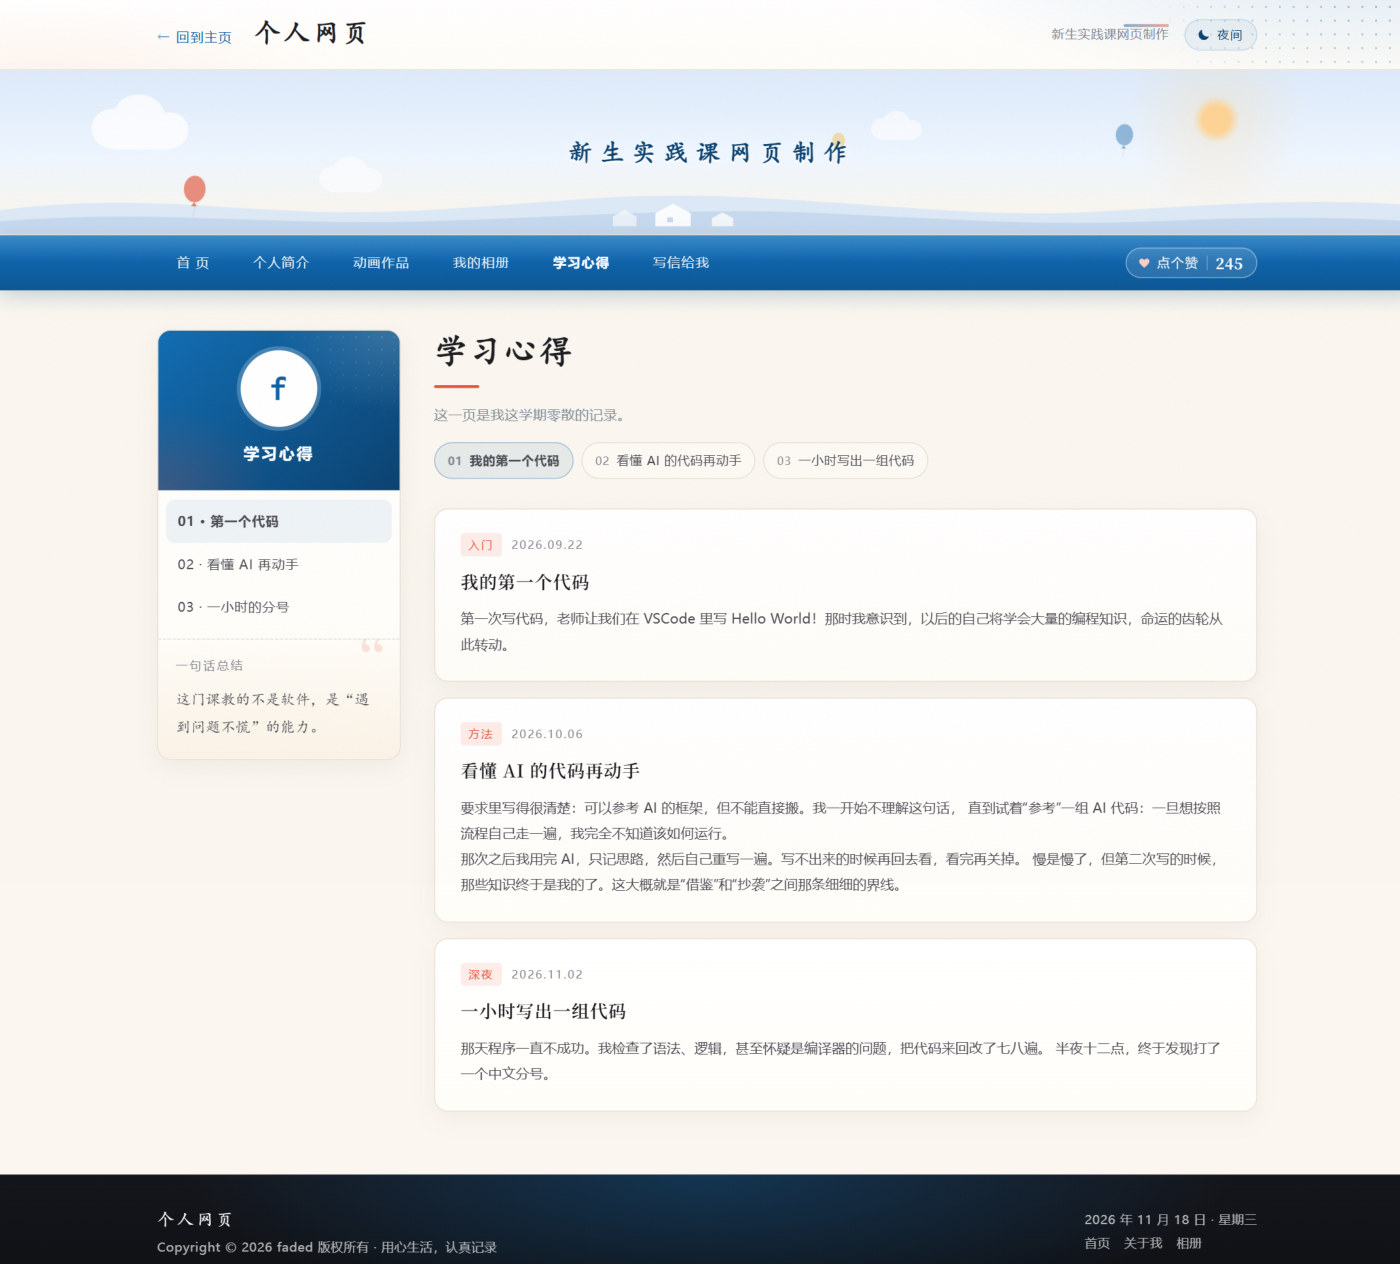
\includegraphics[width=12.8cm]{thoughts.jpg}
  \caption{学习心得页（左侧目录随滚动高亮，顶部为阅读进度环）}
\end{figure}

三篇短文按时间排：第一篇写第一次在编辑器里敲出 Hello World；第二篇写「可以参考 AI 的框架、但不能直接搬」这条要求，以及自己照着走一遍时卡住的那次；第三篇是深夜调程序，来回改了七八遍，最后发现是一个中文分号。

左边有页内目录，阅读时顶部一条进度环；下次打开会问要不要接着读上次断的地方，选「继续」就跳回断点，选「从头」就回到第一段。这个提示只在读过一半以上时才出现，否则每次进来都弹一下，反而烦。页面如图 3-4 所示。

\section{网页设计小结}

问题基本都出在「本地看着好好的，传上去就不对」。

（1）第一次是照片全裂。Dreamweaver 的实时视图里六张图都在，传到 Pages 上全是破图标。原因是我在 \texttt{src} 里写过 \texttt{C:\textbackslash Users\textbackslash ...} 这样的绝对路径，本机当然找得到，服务器上并没有这个盘。改成 \texttt{images/sunset.jpg} 这种相对路径就正常了。后来我把整个文件夹拷到 U 盘、换个目录打开，确认还能显示，才敢再传。

（2）第二次是托管。一开始用 Gitee Pages，还没等页面调顺，它先下线了。转到 GitHub Pages，仓库名从 \texttt{myhouse} 改成 \texttt{homework}，页面里的链接、README 里的地址、页脚的署名全要跟着改一遍。这件事让我第一次觉得，「改个名字」不是小事。推送时还遇到过一次分支搞错：本地推的是 \texttt{master}，站点发布的分支却是 \texttt{main}，推上去半小时网页都没变，最后对着远程分支重新提交才通。

（3）第三次是 404。Pages 会把任何找不到的路径都交给 404.html，但页面在 \texttt{/homework/xxx/yyy} 这样的深层地址下打开时，里面的 \texttt{css/style.css} 仍按相对路径去找，样式就全丢了。解决办法是先用脚本从地址里反推站点根目录，再把样式、脚本和链接都改成从根开始写。还有一处小坑：刚加夜间模式时，刷新会先白一下再变黑，因为样式表加载完才去读本地存储；后来在页面最前面塞了一小段内联脚本，先把主题标记打上，再让样式表进来，就不闪了。

报告这条线也差不多。模板是从群里下的压缩包，直接拖进 Overleaf 新建项目，编译器要手动选 XeLaTeX，不然中文全是方框。名字里的「屾」字 Fandol 字体没有，编译出来是个空框，模板里已经写好了用另一套字体单独补这一个字的办法。正文那些整行的「×」是占位符，得整行删掉再写；我第一次是把文字接在「×」后面，排出来一塌糊涂。图片放在 \texttt{images/} 下用相对路径引，和网页那边是同一个道理。

五页做完回头看，Dreamweaver 其实只负责打字和预览，真正花时间的是布局怎么摆、路径怎么写、出了问题去哪儿找。这些在课上只占半页幻灯片，做的时候却占了一大半时间。

\section{课程的收获和建议}

新生实践课带我初步接触了计算机学科常用的知识和工具，以下按各专题简单总结我的收获与建议。

\subsection{计算机基础知识}

收获：以前对计算机的认识停留在「会用」。这一学期知道了文件在磁盘上是怎么放的、路径为什么分相对和绝对、网页打开时浏览器到底做了哪几件事。建议：这部分多讲一点文件与路径，后面 Office、网页、Git 全要用到，早点讲清楚能少走很多弯路。

\subsection{Windows 及 Office 系列软件}

收获：Word 练的是字效和段落，把《念奴娇》排了一页；Excel 做了一张成绩表，用求平均、按总分排序；PPT 做的是母校郧阳中学，九页，第一次认真调了对齐和母版。建议：Excel 的函数和排序多留一点时间，课上跟着做一遍，课下很容易忘。

\subsection{编程工具 Python}

收获：从缩进开始学，报错看不懂就一行行注释掉试。最大的收获不是会写多少行，而是知道报错信息要先读第一行和最后一行。建议：每节课后留两个十几行就能写完的小题目，比看示例管用。

\subsection{图像设计软件 Photoshop}

收获：学了图层、蒙版、抠图。相册里那六张照片是自己手机拍的，只做了裁切和提亮，没敢大改。建议：多讲一点导出——网页用的图要多大、存成什么格式，这次做相册时尺寸全靠自己试。

\subsection{版本管理软件 Git}

收获：用 SourceTree 提交、推送。第一次看到提交记录一条条排下来，才明白「版本」是什么意思；也是在那时候知道，改坏了可以退回上一个版本。建议：专门讲一次「改坏了怎么退回去」，这个场景最常用，也最能让人放心大胆地改。

\subsection{网页制作 Dreamweaver}

收获：这一节花时间最多，也最像「做东西」。Dreamweaver 的代码提示和实时视图对新手很友好，真正的门槛在布局和部署。建议：把软件操作演示压缩一些，多讲 Flex/Grid 和发布流程；如果能让每个人当场把自己的页面传上去、用手机打开看一眼，印象会比看演示深得多。

总的来说，这门课让我对计算机专业将要学什么有了初步认识，也让我借助 AI 辅助做出了一个真正能访问的个人网站，收获很大。

\end{document}
